\onehalfspacing
\section{Đề số 8}
\graphicspath{{./img/}}
\begin{bt} 
	\hfill
	\begin{enumerate}[a.]
		\item So sánh hai số: $(-5)^{39}$ và $(-2)^{91}$
		\item Chứng minh rằng: Số $\mathrm{A}=11^{\mathrm{n}+2}+12^{2 \mathrm{n}+1}$ chia hết cho 133 , với mọi $\mathrm{n} \in \mathrm{N}$
	\end{enumerate}
	\loigiai{
		\begin{enumerate}
			\item Ta có: $$(-5)^{39}=-5^{39}=-\left(5^3\right)^{13}=-125^{13}$$
			$$
			(-2)^{91}=-2^{91}=-\left(2^7\right)^{13}=-128^{13}
			$$
			Ta thấy: $125^{13}<128^{13} \Rightarrow-125^{13}>-128^{13} \Rightarrow(-5)^{39}>(-2)^{91}$
			\item Ta có: $\mathrm{A}=11^{\mathrm{n}+2}+12^{2 \mathrm{n}+1}=11^2 \cdot 11^{\mathrm{n}}+12 \cdot\left(12^2\right)^{\mathrm{n}}=121 \cdot 11^{\mathrm{n}}+12 \cdot 144^{\mathrm{n}}$ $=(133-12) \cdot 11^{\mathrm{n}}+12 \cdot 144^{\mathrm{n}}=133 \cdot 11^{\mathrm{n}}-12 \cdot 11^{\mathrm{n}}+12 \cdot 144^{\mathrm{n}}$\\[5px] $=133.11^{\mathrm{n}}+12 \cdot\left(144^{\mathrm{n}}-11^{\mathrm{n}}\right)$\\[5px]
			Ta thấy: $133.11^{\text {n}} \vdots 133$
			$$
\left(144^{\mathrm{n}}-11^{\mathrm{n}}\right) \vdots(144-11)=133 \Rightarrow 12 \cdot\left(144^{\mathrm{n}}-11^{\mathrm{n}}\right) \vdots 133
$$
Do đó suy ra: $133.11^{\mathrm{n}}+12 .\left(144^{\mathrm{n}}-11^{\mathrm{n}}\right)$ chia hết cho 133\\[5px]
Vậy: số $\mathrm{A}=11^{\mathrm{n}+2}+12^{2 \mathrm{n}+1}$ chia hết cho 133 , với mọi $\mathrm{n} \in \mathrm{N}$
		\end{enumerate}
	} 
\end{bt}

\begin{bt}
	\hfill
	\begin{enumerate}[a.]
		\item Tìm tất cả các cặp số $(x ; y)$ thỏa mãn: $(2 x-y+7)^{2012}+|x-3|^{2013} \leq 0$
		\item Tìm số tự nhiên $\mathrm{n}$ và chữ số $\mathrm{a}$ biết rằng: $1+2+3+\ldots+n=\overline{a a a}$
	\end{enumerate}
	\loigiai{
		\begin{enumerate}
			\item Ta có: 2012 là số tự nhiên chẵn $\Rightarrow(2 x-y+7)^{2012} \geq 0$ và $|x-3| \geq 0 \\[5px] \Rightarrow|x-3|^{2013} \geq 0$\\[5px]
			Do đó, từ $(2 x-y+7)^{2012}+|x-3|^{2013} \leq 0$\\[5px]
			suy ra: $(2 \mathrm{x}-\mathrm{y}+7)^{2012}=0$ và $|x-3|^{2013}=0$\\[5px]
			$\Rightarrow 2 \mathrm{x}-\mathrm{y}+7=0(1)$ và $\mathrm{x}-3=0(2)$\\[5px]
			Từ (2) $\Rightarrow x=3$\\[5px]
			Từ (1) $\Rightarrow \mathrm{y}=2 \mathrm{x}+7=2.3+7=13$\\[5px]
			Vậy cặp số $(x ; y)$ cần tìm là $(3 ; 13)$
			\item Ta có: $1+2+3+\ldots+n=\frac{n(n+1)}{2}$ và $\overline{a a a}=a .111=a .3 .37$\\[5px]
			Do đó, từ $1+2+3+\ldots+n=\overline{a a a} \\[5px] \Rightarrow n(n+1)=2 \cdot 3 \cdot 37 . a$ \\[5px] $\Rightarrow \mathrm{n}(\mathrm{n}+1)$ chia hết cho số nguyên tố 37\\[5px]
			$\Rightarrow \mathrm{n}$ hoặc $\mathrm{n}+1$ chia hết cho 37 (1)\\[5px]
			Mặt khác: $\frac{n(n+1)}{2}=\overline{a a a} \leq 999\\[5px] \Rightarrow \mathrm{n}(\mathrm{n}+1) \leq 1998 \Rightarrow \mathrm{n}<45$ (2)\\[5px]
			Từ (1) và (2) suy ra hoặc $n=37$, hoặc $n+1=37$\\[5px]
			- Với $\mathrm{n}=37$ thì $\overline{a a a}=\frac{37.38}{2}=703$ (không thỏa)\\[5px]
			- Với $\mathrm{n}+1=37$ thì $\overline{a a a}=\frac{36.37}{2}=666$ (thỏa mãn)\\[5px]
			Vậy $n=36$ và $a=6$.
		\end{enumerate}
	} 
\end{bt}

\begin{bt}
	Ba lớp 7 ở trường K có tất cả 147 học sinh. Nếu đưa $\frac{1}{3}$ số học sinh của lớp $7 \mathrm{~A}_1, \frac{1}{4}$ số học sinh của lớp $7 \mathrm{~A}_2$ và $\frac{1}{5}$ số học sinh của lớp $7 \mathrm{~A}_3$ đi thi học sinh giỏi cấp huyện thì số học sinh còn lại của ba lớp bằng nhau. Tính tổng số học sinh của mỗi lớp 7 ở trường K.
	\loigiai{
		Gọi tổng số học sinh của $7 \mathrm{~A}_1, 7 \mathrm{~A}_2, 7 \mathrm{~A}_3$ lần lượt là $\mathrm{a}, \mathrm{b}, \mathrm{c}\left(\mathrm{a}, \mathrm{b}, \mathrm{c} \in \mathrm{N}^*\right)$\\[5px]
        Theo bài ra ta có : $\mathrm{a}-\frac{1}{3} \mathrm{a}=\mathrm{b}-\frac{1}{4} \mathrm{~b}=\mathrm{c}-\frac{1}{5} \mathrm{c}\left({ }^*\right)$ và $\mathrm{a}+\mathrm{b}+\mathrm{c}=147$ \\[5px] Từ $\left({ }^*\right) \Rightarrow \frac{2 a}{3}=\frac{3 b}{4}=\frac{4 c}{5} \Rightarrow \frac{12 a}{18}=\frac{12 b}{16}=\frac{12 c}{15}\\[5px] \Rightarrow \frac{a}{18}=\frac{b}{16}=\frac{c}{15}$\\[5px]
        Áp dụng tính chất dãy tỷ số bằng nhau ta có :
$$
\frac{a}{18}=\frac{b}{16}=\frac{c}{15}=\frac{a+b+c}{18+16+15}=\frac{147}{49}=3 .
$$
Suy ra: $a=54, b=48, c=45$\\[5px]
Vậy tổng số học sinh của $7 \mathrm{~A}_1, 7 \mathrm{~A}_2$, $7 \mathrm{~A}_3$ lần lượt là 54,48 và 45 .
	} 
\end{bt}

\begin{bt}
	Cho tam giác $\mathrm{ABC}$ có $\hat{A}=3 \hat{B}=6 \hat{C}$.
	\begin{enumerate}[a.]
		\item Tính số đo các góc của tam giác $\mathrm{ABC}$.
		\item Kẻ $\mathrm{AD}$ vuông góc với $\mathrm{BC}$ (D thuộc $\mathrm{BC}$ ). Chứng minh: $\mathrm{AD}<\mathrm{BD}<\mathrm{CD}$.
	\end{enumerate}
	\loigiai{
		$$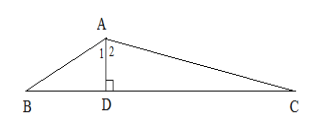
\includegraphics[width=0.55\textwidth]{8-4-lg.png}$$
		\begin{enumerate}
			\item Từ $\hat{A}=3 \hat{B}=6 \hat{C} \Rightarrow \frac{\hat{A}}{6}=\frac{\hat{B}}{2}=\frac{\hat{C}}{1}=\frac{\hat{A}+\hat{B}+\hat{C}}{6+2+1}=\frac{180^{\circ}}{9}=20^{\circ}$\\[5px] 
			$
			\begin{aligned}
				\Rightarrow \hat{A} & =6.20^{\circ}=120^{\circ} \\[5px]
				\hat{B} & =2.20^{\circ}=40^{\circ} \\[5px]
				\hat{C} & =1.20^{\circ}=20^{\circ}
				\end{aligned}
			$
			$\text { Vậy: } \hat{A}=120^{\circ} ; \hat{B}=40^{\circ} ; \hat{C}=20^{\circ}$
		    \item - Trong $\triangle \mathrm{ACD}$ có\\[5px]
			$
			\begin{aligned}
			A \hat{D} C=90^{\circ} ; \hat{C}=20^{\circ} & \Rightarrow \hat{A}_2=70^{\circ} \\[5px]
			& \Rightarrow \hat{A}_1=50^{\circ}
			\end{aligned}
			$\\[5px]
			- Xét $\triangle \mathrm{ADB}$ có $\hat{B}=40^{\circ}<\hat{A}_1=50^{\circ} \Rightarrow A D<B D$ (1)\\[5px]
			- Xét $\triangle \mathrm{ABC}$ có $\left.\hat{B}=40^{\circ}>\hat{C}=20^{\circ} \Rightarrow A B<A C \Rightarrow A B^2<A C^2{ }^*\right)$\\[5px]
			- Áp dụng định lý Pytago cho hai tam giác vuông $\mathrm{ADB}$ và $\mathrm{ADC}$ có: $\mathrm{AB}^2=\mathrm{AD}^2+\mathrm{BD}^2$ và $\mathrm{AC}^2=\mathrm{AD}^2+\mathrm{CD}^2$\\[5px]
			Do đó, từ $\left(^*\right) \Rightarrow \mathrm{AD}^2+\mathrm{BD}^2<\mathrm{AD}^2+\mathrm{CD}^2$
			$\\[5px]
			\Rightarrow \mathrm{BD}^2<\mathrm{CD}^2 \Rightarrow \mathrm{BD}<\mathrm{CD} \text { (2) }
			$\\[5px]
			Từ (1) và $(2) \Rightarrow \mathrm{AD}<\mathrm{BD}<\mathrm{CD}$
		\end{enumerate}
	}
\end{bt}

\begin{bt}
	Cho tam giác $A B C$ cân ở $A$. Trên cạnh $A B$ lấy điểm $M$, trên tia đối của tia CA lấy điểm $\mathrm{N}$ sao cho $\mathrm{AM}+\mathrm{AN}=2 \mathrm{AB}$.
	\begin{enumerate}[a.]
		\item Chứng minh rằng: $\mathrm{BM}=\mathrm{CN}$
		\item Chứng minh rằng: $\mathrm{BC}$ đi qua trung điểm của đoạn thẳng $\mathrm{MN}$.
		\item Đường trung trực của $\mathrm{MN}$ và tia phân giác của góc $\mathrm{BAC}$ cắt nhau tại $\mathrm{K}$. Chứng minh rằng: $\mathrm{KC} \perp \mathrm{AC}$.
	\end{enumerate}
	\loigiai{
		$$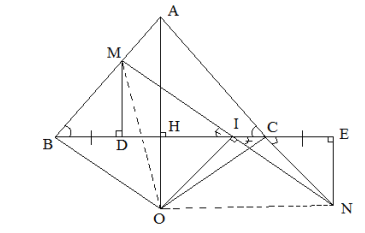
\includegraphics[width=0.55\textwidth]{4-4-lg.png}$$
		\begin{enumerate}
			\item Theo giả thiết, ta có:\\[5px]
			$
			\begin{aligned}
			& 2 \mathrm{AB}=\mathrm{AB}+\mathrm{AB}=\mathrm{AB}+\mathrm{AM}+\mathrm{BM} \\[5px]
			& \mathrm{AM}+\mathrm{AN}=\mathrm{AM}+\mathrm{AC}+\mathrm{CN} \\[5px]
			& \Delta \mathrm{ABC} \text { cân ở } \mathrm{A} \Rightarrow \mathrm{AB}=\mathrm{AC} \\[5px]
			& \text { Do đó, từ } \mathrm{AM}+\mathrm{AN}=2 \mathrm{AB} \\[5px]
			& \Rightarrow \mathrm{BM}=\mathrm{CN}
			\end{aligned}
			$
			\item Qua M kẽ $M E / / A C(E \in B C)$
			$\triangle \mathrm{ABC}$ cân ở $\mathrm{A} \Rightarrow \triangle \mathrm{BME}$ cân ở $\mathrm{M} \Rightarrow \mathrm{EM}=\mathrm{BM}=\mathrm{CN}$ $\Rightarrow \Delta \mathrm{MEI}=\Delta \mathrm{NCI}(\mathrm{g}-\mathrm{c}-\mathrm{g}) \Rightarrow \mathrm{IM}=\mathrm{IN}$\\[5px]
			Vậy: BC đi qua trung điểm của MN.
			\item $+\mathrm{K}$ thuộc đường trung trực của $\mathrm{MN} \Rightarrow \mathrm{KM}=\mathrm{KN}$ (1)\\[5px]
			$+\triangle \mathrm{ABK}=\Delta \mathrm{ACK}(\mathrm{c}-\mathrm{g}-\mathrm{c}) \Rightarrow \mathrm{KB}=\mathrm{KC} \text{ (2) } ; A \hat{B K}=A \hat{C} K\left(^*\right)$\\[5px]
			+ Kết quả câu c/m câu a $\mathrm{BM}=\mathrm{CN}$ (3)\\[5px]
			+ Từ (1), (2) và (3) $\Rightarrow \Delta \mathrm{BMK}=\Delta \mathrm{CNK}(\mathrm{c}-\mathrm{c}-\mathrm{c}) \Rightarrow A \hat{B} K=N \hat{C K} \quad\left({ }^{* *}\right)$\\[5px]
			+ Từ $\left({ }^*\right)$ và $\left({ }^{* *}\right) \Rightarrow A \hat{C} K=N \hat{C} K=\frac{180^{\circ}}{2}=90^{\circ} \Rightarrow \mathrm{KC} \perp \mathrm{AN}$
		\end{enumerate}
	}
\end{bt}